% FAS2AlgorithmsOnGraphsTikZ-001
% Asset type: TikZ diagram
% Topic: FAS2-ALGGRAPH Algorithms on graphs
% Purpose: Flow chart for smallest-value algorithm.
\documentclass[tikz,border=8pt]{standalone}
\usepackage{amsmath}
\usepackage{xcolor}
\usetikzlibrary{arrows.meta,positioning,shapes.geometric,shapes.misc,calc}
\definecolor{Canvas}{HTML}{FAF9F6}
\definecolor{Panel}{HTML}{FFFFF0}
\definecolor{Line}{HTML}{E5E5EA}
\definecolor{Accent}{HTML}{D4AF37}
\definecolor{Soft}{HTML}{FBEFEF}
\definecolor{Text}{HTML}{2C2C2E}
\begin{document}
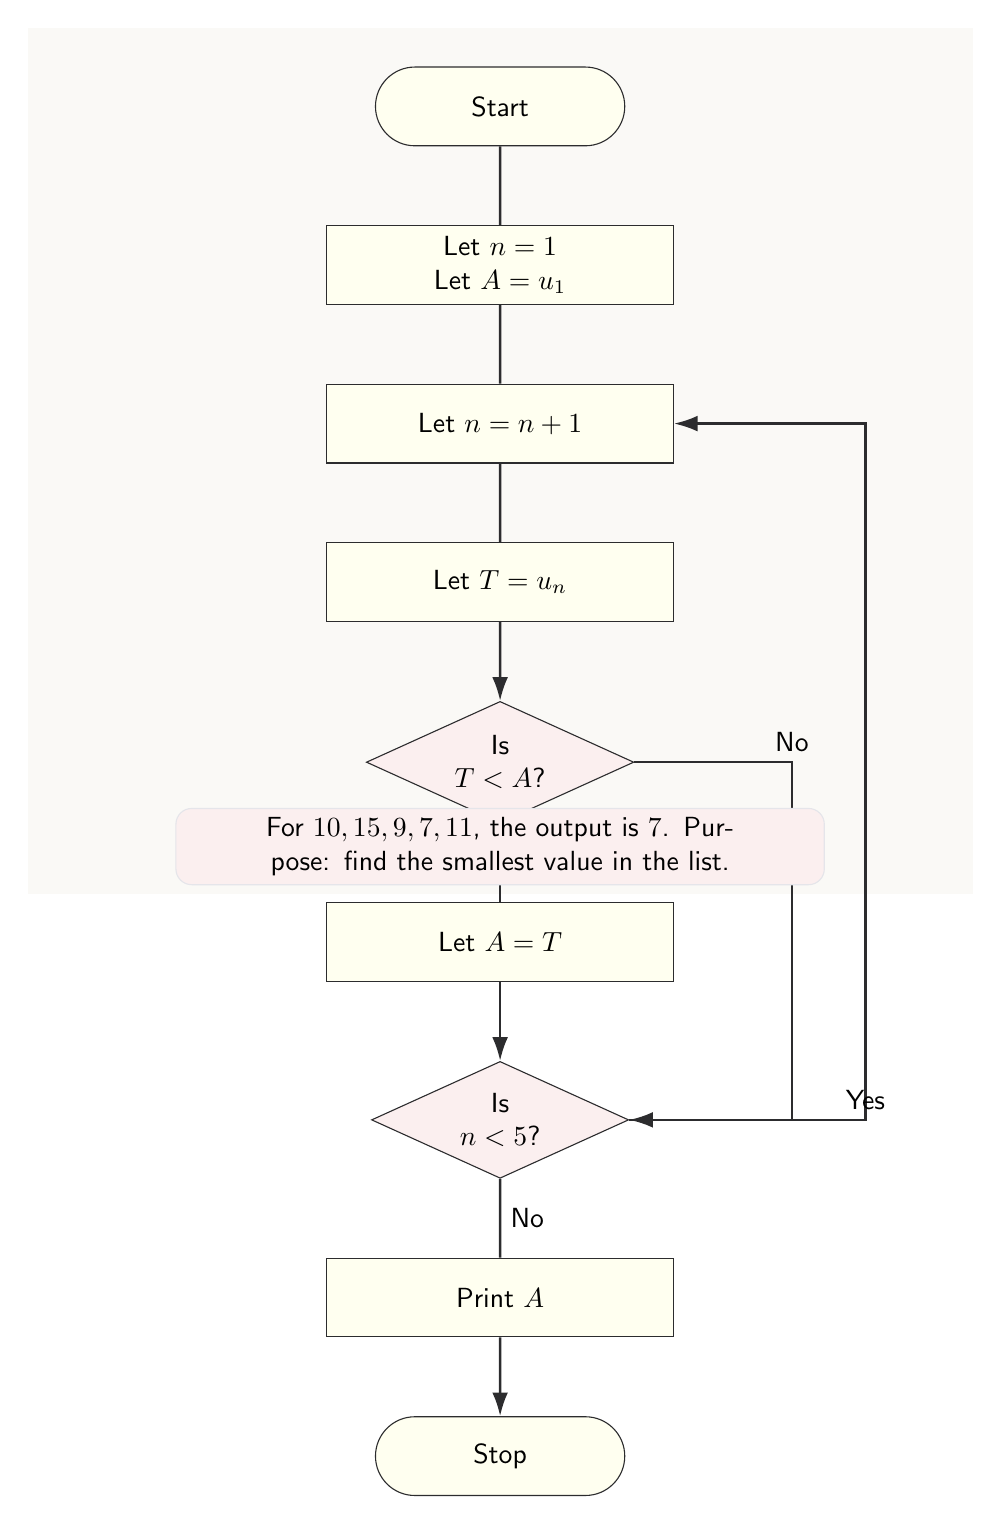
\begin{tikzpicture}[font=\sffamily,>=Latex,node distance=10mm,flowline/.style={draw=Text,line width=0.9pt,-{Latex[length=3mm,width=2mm]}},startstop/.style={rounded rectangle,draw=Text,fill=Panel,minimum width=34mm,minimum height=10mm,align=center},process/.style={rectangle,draw=Text,fill=Panel,minimum width=44mm,minimum height=10mm,align=center},decision/.style={diamond,draw=Text,fill=Soft,aspect=2.2,align=center}]
\fill[Canvas] (-6,-9) rectangle (6,2);
\node[startstop] (start) at (0,1) {Start};
\node[process,below=of start] (init) {Let \(n=1\)\\Let \(A=u_1\)};
\node[process,below=of init] (inc) {Let \(n=n+1\)};
\node[process,below=of inc] (t) {Let \(T=u_n\)};
\node[decision,below=of t] (test) {Is\\ \(T<A\)?};
\node[process,below=of test] (update) {Let \(A=T\)};
\node[decision,below=of update] (ncheck) {Is\\ \(n<5\)?};
\node[process,below=of ncheck] (out) {Print \(A\)};
\node[startstop,below=of out] (stop) {Stop};
\draw[flowline] (start)--(init)--(inc)--(t)--(test);
\draw[flowline] (test)--node[right]{Yes}(update)--(ncheck);
\draw[flowline] (test.east)--++(2,0) node[above]{No} |- (ncheck.east);
\draw[flowline] (ncheck.east)--++(3,0) node[above]{Yes} |- (inc.east);
\draw[flowline] (ncheck)--node[right]{No}(out)--(stop);
\node[draw=Line,fill=Soft,rounded corners=2mm,text width=80mm,align=center] at (0,-8.4) {For \(10,15,9,7,11\), the output is \(7\). Purpose: find the smallest value in the list.};
\end{tikzpicture}
\end{document}
